\chapter{Introduction}\label{sec:intro}
\begin{flushright}{\slshape    
The most important contribution of management in the 20th century\\
was to increase manual worker productivity fifty-fold.\\
The most important contribution of management in the 21st century\\
will be to increase knowledge worker productivity\\
— hopefully by the same percentage} \\ \medskip
--- Peter Drucker~\cite{drucker1999}
\end{flushright}

When Peter Drucker became aware that the level of automation in manual labour was rising faster than that in knowledge work, he said these words at the end of the $20^{th}$ century in 1999. Between both types of work lies a pronounced difference: The course of manual work is determined by physical laws, while the course of knowledge work requires one to "think for a living" and allows for flexible execution of the work.

Now, 20 years later, numerous knowledge repositories and assistance systems exist for knowledge workers to help in making decisions more informed and faster. These assistance systems log the course of every case, i.e. every instance of a process, until its completion.\\

This thesis leverages these logs and presents a step towards actively assisting the knowledge worker by predicting the activity which would usually be executed next in the context of a trace. These predictions are derived from a special type of neural network.\\

\begin{figure}
    \centering
    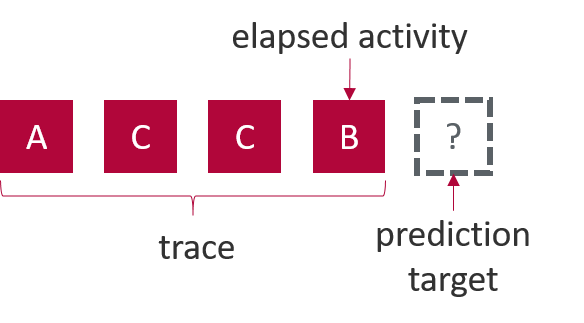
\includegraphics[width=\textwidth]{gfx/next-activity.png}
    \caption{Predicting the next activity}
    \label{fig:next-activity-prediction}
\end{figure}

The application of Predictive Analytics in Process Science is fairly recent, and is generally referred to as Predictive Process Monitoring (see \autoref{chap:background}). As it is a new domain, only a small number of publications have addressed the next-activity prediction problem. Much more work exists on a typical prediction problem for traditional business processes: prediction of predicate conformance or completion time (see \autoref{fig:next-activity-prediction}). Furthermore, the fact that no benchmarking dataset for this kind of problem has yet been established, although the datasets of the Business Process Intelligence Competition (BPIC)~\cite{BPIC2011, BPIC2012, BPIC2017} have often been used. And lastly, this type of prediction problem has not been related to similar problems in domains in which more expertise has been collected.\\

This thesis addresses these facts by proposing a revised prediction model that was inspired by predictive models applied in the area of Natural Language Processing (NLP). This approach is tested on the datasets of BPIC2011 and BPIC2012 and compared to two implementations taken from the following papers, thus allowing direct comparability:

\begin{enumerate}
    \item \textit{A Deep Learning Approach for Predicting Process Behaviour at Runtime} by Evermann et al.~\cite{evermann2016} \item\textit{Deep Learning Process Prediction with Discrete and Continuous Data Features} by Schönig et al.~\cite{schoenig2018}.
\end{enumerate}

These two works have been identified as successively building upon each other, and the predictive models were reverse-engineered in close collaboration with the authors.

<ACTIVITY><DATA><ENGINEERED FEATURES>

\section{Research questions}\label{sec:intro:objective}
\todo[inline]{Does including SP-2 information lead to improved predictions?}
\todo[inline]{Does more data lead to better predictions?}

In my thesis, I want to investigate the synergies of combining the aforementioned approach of Francescomarino et al. for learning data clustering with LSTM neural networks as per Evermann et al. Case data attributes shall be used during model training and prediction, as Polato et al. \cite{polato2014} and Schönig et al. \cite{schoenig2018} demonstrated their usefulness.

This would contribute to a field of research which is currently being explored and where LSTM networks have been applied successfully on prediction problems with long-term dependencies \cite{evermann2016, tax2017, schoenig2018, graves2005}.

%Furthermore, I want to investigate how much the accuracy of current LSTM approaches is improved if the learning data is clustered.
Furthermore, I want to determine how historical case log data is prepared best for learning, as only Schönig et al. have written a small subsection on this \cite{schoenig2018}.
If time permits, I also want to investigate the potential of ensembles within this context, as they can potentially enlighten the user about the reason for a prediction.
With neural networks it is hard to comprehend the reasons behind a prediction.
Other types of models deliver better comprehensibility.

Throughout the document I will strive to meet recently demanded machine learning paper quality criteria \cite{lipton2018}.

The performance of the combined approaches shall be evaluated against the data from the Business Process Intelligence Challenges (BPIC) 2011, 2012 and 2017 \cite{BPIC2011, BPIC2012, BPIC2017}. This allows for comparison with the results of Francescomarino et al., Evermann et al., Tax et al. and Schönig et al. \cite{francescomarino2018, evermann2016, tax2017, schoenig2018}.
The next steps and an approximate timeframe are shown in the table below:\\[1em]

\todo[inline]{taylorism}

\textbf{Does including subsequence information improve prediction quality}

\textbf{Does more data lead to better predictions? If so, which criteria must it present?}

Adaptive Case Management (ACM)

1. establish baseline mimicking evermann and schönig
enhance with prefixspan-mined features and sp-k encoded features
measure difference
measure earliness

Three pillars to my work
Evermann
Schönig
Shibata

Combination
Publish benchmark in comparison to other precisions and approaches

\section{Thesis Structure}\label{sec:intro:structure}


